\documentclass{beamer}

\usepackage[utf8]{inputenc}
\usepackage{default}
\usepackage{tikz}
\usepackage{color}

\begin{document}
\title{Fast Nearest Neighbour Classification}
\author{Gordon Lesti}
\date{17.07.2015}

\frame{\titlepage}
\frame{\frametitle{Inhaltsverzeichnis}\tableofcontents}

\section{Einleitung}

\subsection{Problem}
\begin{frame}
 \frametitle{Nearest-Neighbor Searching}
 \begin{block}{Gegeben}
   \begin{itemize}
    \item Menge $\mathbb{U}$
    \item Abstandsmaß $d$ auf $\mathbb{U}$, mit $d: \mathbb{U} \times \mathbb{U} \to \mathbb{R}$
    \item Menge $S \subset \mathbb{U}$ der Größe $n$
    \item Anfragepunkt $q \in \mathbb{U}$
  \end{itemize}
 \end{block}
 \begin{block}{Gesucht}
    \begin{itemize}
     \item $a \in S$, mit $d(q, a) \le d(q, x)$ f\"ur alle $x \in S$
    \end{itemize}
 \end{block}
\end{frame}

\subsection{Anwendung}
\begin{frame}
 \frametitle{Anwendung}
 \begin{itemize}
 \item density estimation
 \item pattern recognition
 \item object recognition
 \item data clustering
 \item function approximation
 \item vector quantization
\end{itemize}
\end{frame}

\section{L\"osungen}

\subsection{Vollsuche}
\begin{frame}
 \frametitle{Vollsuche}
 \begin{itemize}
  \item Berechne $d(q, x)$ f\"ur alle $x \in S$
  \item W\"ahle $a \in S$, mit $d(q, a) \le d(q, x)$ f\"ur alle $x \in S$
 \end{itemize}
\end{frame}

% Beispiel1 Datenpunkte
\begin{frame}{Vollsuche}{Beispiel}
 \begin{columns}[T]
  \begin{column}{.35\textwidth}
    $\mathbb{U} = \mathbb{R}^2$
    \begin{block}{Datenpunkte}
      $x_1 = (3, 3)$\\
      $x_2 = (-1, 2)$\\
      $x_3 = (-4, -4)$\\
      $x_4 = (0, -1)$\\
      $x_5 = (4, -3)$
    \end{block}
  \end{column}
  \begin{column}{.6\textwidth}
     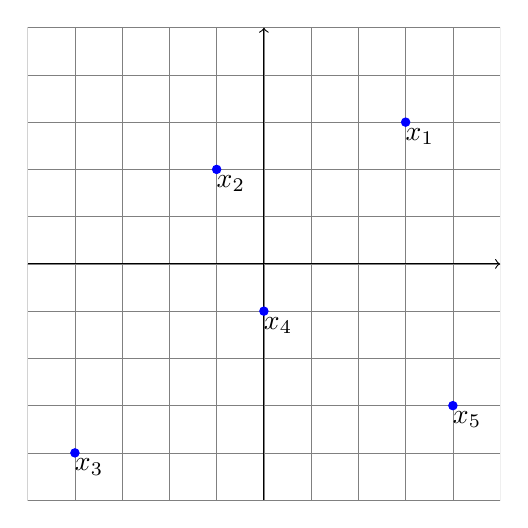
\begin{tikzpicture}[%
      scale=0.6,
      ]
      \clip (-5.0,-5.0) rectangle (5.0,5.0);
      \draw [help lines] (0,0) grid (6,5);
      \draw [help lines] (-6,0) grid (0,5);
      \draw [help lines] (0,-6) grid (6,0);
      \draw [help lines] (-6,-6) grid (0,0);
      \draw [color=black,->] (-5.0,0) -- (5.0,0);
      \draw [color=black,->] (0,-5.0) -- (0,5.0);
      
      \filldraw [color={rgb:red,0;green,0;blue,255}] (3,3) circle (2.5pt );
      \filldraw [color={rgb:red,0;green,0;blue,255}] (-1,2) circle (2.5pt );
      \filldraw [color={rgb:red,0;green,0;blue,255}] (-4,-4) circle (2.5pt );
      \filldraw [color={rgb:red,0;green,0;blue,255}] (0,-1) circle (2.5pt );
      \filldraw [color={rgb:red,0;green,0;blue,255}] (4,-3) circle (2.5pt );
      
      \node at (3.3,2.7) {$x_1$};
      \node at (-0.7,1.7) {$x_2$};
      \node at (-3.7,-4.3) {$x_3$};
      \node at (0.3,-1.3) {$x_4$};
      \node at (4.3,-3.3) {$x_5$};
      \end{tikzpicture}
  \end{column}
 \end{columns}
\end{frame}

% Beispiel1 Anfragepunkt
\begin{frame}{Vollsuche}{Beispiel}
 \begin{columns}[T]
  \begin{column}{.35\textwidth}
    $\mathbb{U} = \mathbb{R}^2$
    \begin{block}{Datenpunkte}
      $x_1 = (3, 3)$\\
      $x_2 = (-1, 2)$\\
      $x_3 = (-4, -4)$\\
      $x_4 = (0, -1)$\\
      $x_5 = (4, -3)$
    \end{block}
    \begin{block}{Anfragepunkt}
      $q = (2, 1)$
    \end{block}
  \end{column}
  \begin{column}{.6\textwidth}
     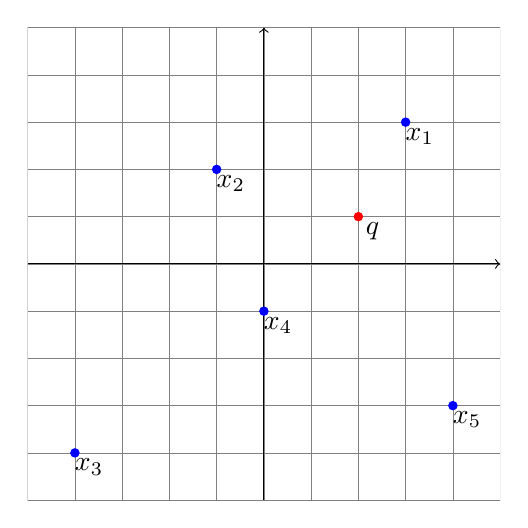
\begin{tikzpicture}[%
      scale=0.6,
      ]
      \clip (-5.0,-5.0) rectangle (5.0,5.0);
      \draw [help lines] (0,0) grid (6,5);
      \draw [help lines] (-6,0) grid (0,5);
      \draw [help lines] (0,-6) grid (6,0);
      \draw [help lines] (-6,-6) grid (0,0);
      \draw [color=black,->] (-5.0,0) -- (5.0,0);
      \draw [color=black,->] (0,-5.0) -- (0,5.0);
      
      \filldraw [color={rgb:red,0;green,0;blue,255}] (3,3) circle (2.5pt );
      \filldraw [color={rgb:red,0;green,0;blue,255}] (-1,2) circle (2.5pt );
      \filldraw [color={rgb:red,0;green,0;blue,255}] (-4,-4) circle (2.5pt );
      \filldraw [color={rgb:red,0;green,0;blue,255}] (0,-1) circle (2.5pt );
      \filldraw [color={rgb:red,0;green,0;blue,255}] (4,-3) circle (2.5pt );
      
      \filldraw [color={rgb:red,255;green,0;blue,0}] (2,1) circle (2.5pt );
      
      \node at (3.3,2.7) {$x_1$};
      \node at (-0.7,1.7) {$x_2$};
      \node at (-3.7,-4.3) {$x_3$};
      \node at (0.3,-1.3) {$x_4$};
      \node at (4.3,-3.3) {$x_5$};
      
      \node at (2.3,0.7) {$q$};
      \end{tikzpicture}
  \end{column}
 \end{columns}
\end{frame}

% Beispiel1 Abstand x1
\begin{frame}{Vollsuche}{Beispiel}
 \begin{columns}[T]
  \begin{column}{.35\textwidth}
    \begin{block}{Ergebnis}
      $d(q, x_1) \approx 2.236$
    \end{block}
  \end{column}
  \begin{column}{.6\textwidth}
     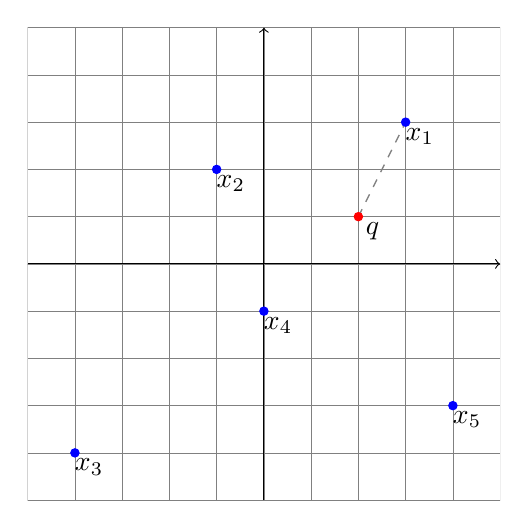
\begin{tikzpicture}[%
      scale=0.6,
      ]
      \clip (-5.0,-5.0) rectangle (5.0,5.0);
      \draw [help lines] (0,0) grid (6,5);
      \draw [help lines] (-6,0) grid (0,5);
      \draw [help lines] (0,-6) grid (6,0);
      \draw [help lines] (-6,-6) grid (0,0);
      \draw [color=black,->] (-5.0,0) -- (5.0,0);
      \draw [color=black,->] (0,-5.0) -- (0,5.0);
      
      \draw[color=gray, line width=0.5pt, dashed] (2,1) -- (3,3);
      
      \filldraw [color={rgb:red,0;green,0;blue,255}] (3,3) circle (2.5pt );
      \filldraw [color={rgb:red,0;green,0;blue,255}] (-1,2) circle (2.5pt );
      \filldraw [color={rgb:red,0;green,0;blue,255}] (-4,-4) circle (2.5pt );
      \filldraw [color={rgb:red,0;green,0;blue,255}] (0,-1) circle (2.5pt );
      \filldraw [color={rgb:red,0;green,0;blue,255}] (4,-3) circle (2.5pt );
      
      \filldraw [color={rgb:red,255;green,0;blue,0}] (2,1) circle (2.5pt );
      
      \node at (3.3,2.7) {$x_1$};
      \node at (-0.7,1.7) {$x_2$};
      \node at (-3.7,-4.3) {$x_3$};
      \node at (0.3,-1.3) {$x_4$};
      \node at (4.3,-3.3) {$x_5$};
      
      \node at (2.3,0.7) {$q$};
      \end{tikzpicture}
  \end{column}
 \end{columns}
\end{frame}

% Beispiel1 Abstand x2
\begin{frame}{Vollsuche}{Beispiel}
 \begin{columns}[T]
  \begin{column}{.35\textwidth}
    \begin{block}{Ergebnis}
      $d(q, x_1) \approx 2.236$\\
      $d(q, x_2) \approx 3.162$
    \end{block}
  \end{column}
  \begin{column}{.6\textwidth}
     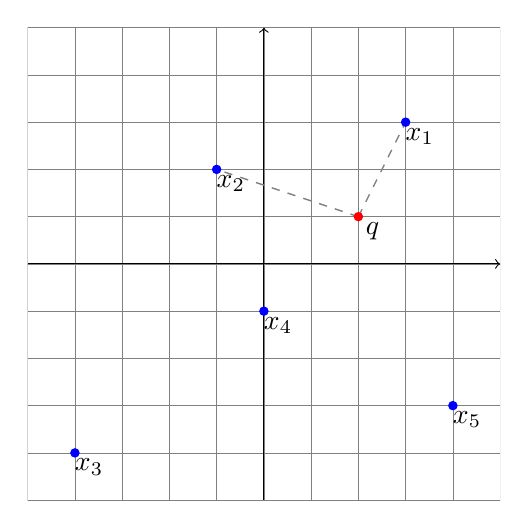
\begin{tikzpicture}[%
      scale=0.6,
      ]
      \clip (-5.0,-5.0) rectangle (5.0,5.0);
      \draw [help lines] (0,0) grid (6,5);
      \draw [help lines] (-6,0) grid (0,5);
      \draw [help lines] (0,-6) grid (6,0);
      \draw [help lines] (-6,-6) grid (0,0);
      \draw [color=black,->] (-5.0,0) -- (5.0,0);
      \draw [color=black,->] (0,-5.0) -- (0,5.0);
      
      \draw[color=gray, line width=0.5pt, dashed] (2,1) -- (3,3);
      \draw[color=gray, line width=0.5pt, dashed] (2,1) -- (-1,2);
      
      \filldraw [color={rgb:red,0;green,0;blue,255}] (3,3) circle (2.5pt );
      \filldraw [color={rgb:red,0;green,0;blue,255}] (-1,2) circle (2.5pt );
      \filldraw [color={rgb:red,0;green,0;blue,255}] (-4,-4) circle (2.5pt );
      \filldraw [color={rgb:red,0;green,0;blue,255}] (0,-1) circle (2.5pt );
      \filldraw [color={rgb:red,0;green,0;blue,255}] (4,-3) circle (2.5pt );
      
      \filldraw [color={rgb:red,255;green,0;blue,0}] (2,1) circle (2.5pt );
      
      \node at (3.3,2.7) {$x_1$};
      \node at (-0.7,1.7) {$x_2$};
      \node at (-3.7,-4.3) {$x_3$};
      \node at (0.3,-1.3) {$x_4$};
      \node at (4.3,-3.3) {$x_5$};
      
      \node at (2.3,0.7) {$q$};
      \end{tikzpicture}
  \end{column}
 \end{columns}
\end{frame}

% Beispiel1 Abstand x3
\begin{frame}{Vollsuche}{Beispiel}
 \begin{columns}[T]
  \begin{column}{.35\textwidth}
    \begin{block}{Ergebnis}
      $d(q, x_1) \approx 2.236$\\
      $d(q, x_2) \approx 3.162$\\
      $d(q, x_3) \approx 7.810$
    \end{block}
  \end{column}
  \begin{column}{.6\textwidth}
     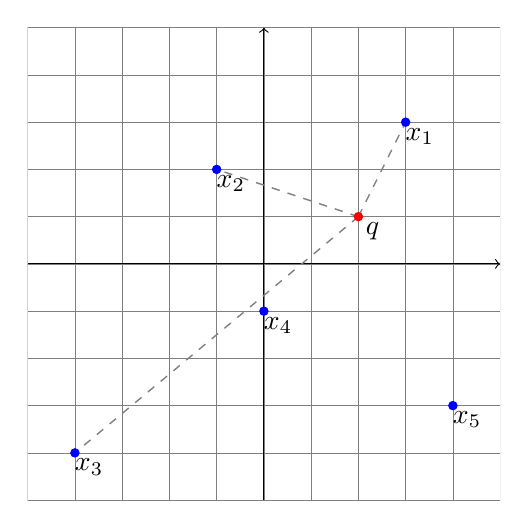
\begin{tikzpicture}[%
      scale=0.6,
      ]
      \clip (-5.0,-5.0) rectangle (5.0,5.0);
      \draw [help lines] (0,0) grid (6,5);
      \draw [help lines] (-6,0) grid (0,5);
      \draw [help lines] (0,-6) grid (6,0);
      \draw [help lines] (-6,-6) grid (0,0);
      \draw [color=black,->] (-5.0,0) -- (5.0,0);
      \draw [color=black,->] (0,-5.0) -- (0,5.0);
      
      \draw[color=gray, line width=0.5pt, dashed] (2,1) -- (3,3);
      \draw[color=gray, line width=0.5pt, dashed] (2,1) -- (-1,2);
      \draw[color=gray, line width=0.5pt, dashed] (2,1) -- (-4,-4);
      
      \filldraw [color={rgb:red,0;green,0;blue,255}] (3,3) circle (2.5pt );
      \filldraw [color={rgb:red,0;green,0;blue,255}] (-1,2) circle (2.5pt );
      \filldraw [color={rgb:red,0;green,0;blue,255}] (-4,-4) circle (2.5pt );
      \filldraw [color={rgb:red,0;green,0;blue,255}] (0,-1) circle (2.5pt );
      \filldraw [color={rgb:red,0;green,0;blue,255}] (4,-3) circle (2.5pt );
      
      \filldraw [color={rgb:red,255;green,0;blue,0}] (2,1) circle (2.5pt );
      
      \node at (3.3,2.7) {$x_1$};
      \node at (-0.7,1.7) {$x_2$};
      \node at (-3.7,-4.3) {$x_3$};
      \node at (0.3,-1.3) {$x_4$};
      \node at (4.3,-3.3) {$x_5$};
      
      \node at (2.3,0.7) {$q$};
      \end{tikzpicture}
  \end{column}
 \end{columns}
\end{frame}

% Beispiel1 Abstand x4
\begin{frame}{Vollsuche}{Beispiel}
 \begin{columns}[T]
  \begin{column}{.35\textwidth}
    \begin{block}{Ergebnis}
      $d(q, x_1) \approx 2.236$\\
      $d(q, x_2) \approx 3.162$\\
      $d(q, x_3) \approx 7.810$\\
      $d(q, x_4) \approx 2.828$
    \end{block}
  \end{column}
  \begin{column}{.6\textwidth}
     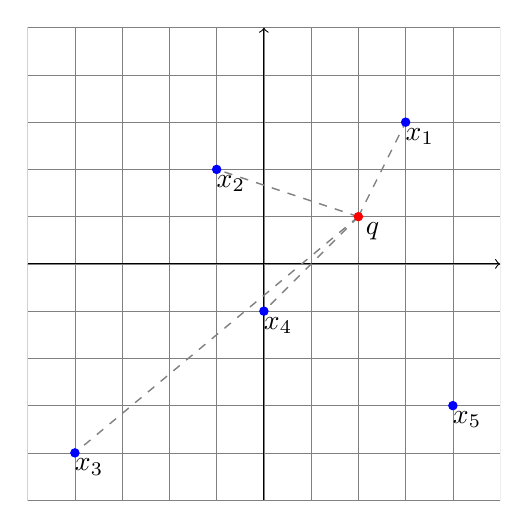
\begin{tikzpicture}[%
      scale=0.6,
      ]
      \clip (-5.0,-5.0) rectangle (5.0,5.0);
      \draw [help lines] (0,0) grid (6,5);
      \draw [help lines] (-6,0) grid (0,5);
      \draw [help lines] (0,-6) grid (6,0);
      \draw [help lines] (-6,-6) grid (0,0);
      \draw [color=black,->] (-5.0,0) -- (5.0,0);
      \draw [color=black,->] (0,-5.0) -- (0,5.0);
      
      \draw[color=gray, line width=0.5pt, dashed] (2,1) -- (3,3);
      \draw[color=gray, line width=0.5pt, dashed] (2,1) -- (-1,2);
      \draw[color=gray, line width=0.5pt, dashed] (2,1) -- (-4,-4);
      \draw[color=gray, line width=0.5pt, dashed] (2,1) -- (0,-1);
      
      \filldraw [color={rgb:red,0;green,0;blue,255}] (3,3) circle (2.5pt );
      \filldraw [color={rgb:red,0;green,0;blue,255}] (-1,2) circle (2.5pt );
      \filldraw [color={rgb:red,0;green,0;blue,255}] (-4,-4) circle (2.5pt );
      \filldraw [color={rgb:red,0;green,0;blue,255}] (0,-1) circle (2.5pt );
      \filldraw [color={rgb:red,0;green,0;blue,255}] (4,-3) circle (2.5pt );
      
      \filldraw [color={rgb:red,255;green,0;blue,0}] (2,1) circle (2.5pt );
      
      \node at (3.3,2.7) {$x_1$};
      \node at (-0.7,1.7) {$x_2$};
      \node at (-3.7,-4.3) {$x_3$};
      \node at (0.3,-1.3) {$x_4$};
      \node at (4.3,-3.3) {$x_5$};
      
      \node at (2.3,0.7) {$q$};
      \end{tikzpicture}
  \end{column}
 \end{columns}
\end{frame}

% Beispiel1 Abstand x5
\begin{frame}{Vollsuche}{Beispiel}
 \begin{columns}[T]
  \begin{column}{.35\textwidth}
    \begin{block}{Ergebnis}
      $d(q, x_1) \approx 2.236$\\
      $d(q, x_2) \approx 3.162$\\
      $d(q, x_3) \approx 7.810$\\
      $d(q, x_4) \approx 2.828$\\
      $d(q, x_5) \approx 4.472$
    \end{block}
  \end{column}
  \begin{column}{.6\textwidth}
     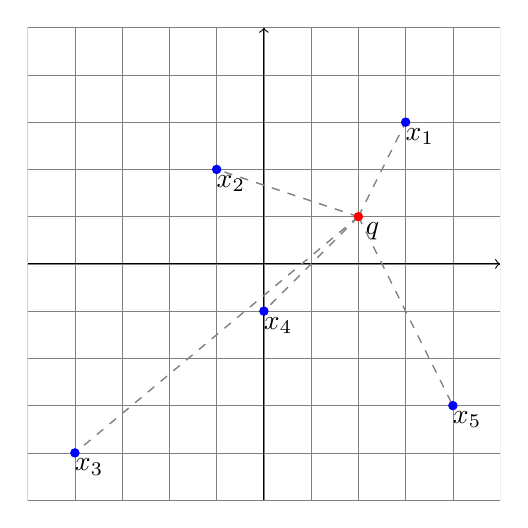
\begin{tikzpicture}[%
      scale=0.6,
      ]
      \clip (-5.0,-5.0) rectangle (5.0,5.0);
      \draw [help lines] (0,0) grid (6,5);
      \draw [help lines] (-6,0) grid (0,5);
      \draw [help lines] (0,-6) grid (6,0);
      \draw [help lines] (-6,-6) grid (0,0);
      \draw [color=black,->] (-5.0,0) -- (5.0,0);
      \draw [color=black,->] (0,-5.0) -- (0,5.0);
      
      \draw[color=gray, line width=0.5pt, dashed] (2,1) -- (3,3);
      \draw[color=gray, line width=0.5pt, dashed] (2,1) -- (-1,2);
      \draw[color=gray, line width=0.5pt, dashed] (2,1) -- (-4,-4);
      \draw[color=gray, line width=0.5pt, dashed] (2,1) -- (0,-1);
      \draw[color=gray, line width=0.5pt, dashed] (2,1) -- (4,-3);
      
      \filldraw [color={rgb:red,0;green,0;blue,255}] (3,3) circle (2.5pt );
      \filldraw [color={rgb:red,0;green,0;blue,255}] (-1,2) circle (2.5pt );
      \filldraw [color={rgb:red,0;green,0;blue,255}] (-4,-4) circle (2.5pt );
      \filldraw [color={rgb:red,0;green,0;blue,255}] (0,-1) circle (2.5pt );
      \filldraw [color={rgb:red,0;green,0;blue,255}] (4,-3) circle (2.5pt );
      
      \filldraw [color={rgb:red,255;green,0;blue,0}] (2,1) circle (2.5pt );
      
      \node at (3.3,2.7) {$x_1$};
      \node at (-0.7,1.7) {$x_2$};
      \node at (-3.7,-4.3) {$x_3$};
      \node at (0.3,-1.3) {$x_4$};
      \node at (4.3,-3.3) {$x_5$};
      
      \node at (2.3,0.7) {$q$};
      \end{tikzpicture}
  \end{column}
 \end{columns}
\end{frame}

% Beispiel1 Ergebnis
\begin{frame}{Vollsuche}{Beispiel}
 \begin{columns}[T]
  \begin{column}{.35\textwidth}
    \begin{block}{Ergebnis}
      \textcolor{green}{$d(q, x_1) \approx 2.236$}\\
      $d(q, x_2) \approx 3.162$\\
      $d(q, x_3) \approx 7.810$\\
      $d(q, x_4) \approx 2.828$\\
      $d(q, x_5) \approx 4.472$
    \end{block}
  \end{column}
  \begin{column}{.6\textwidth}
     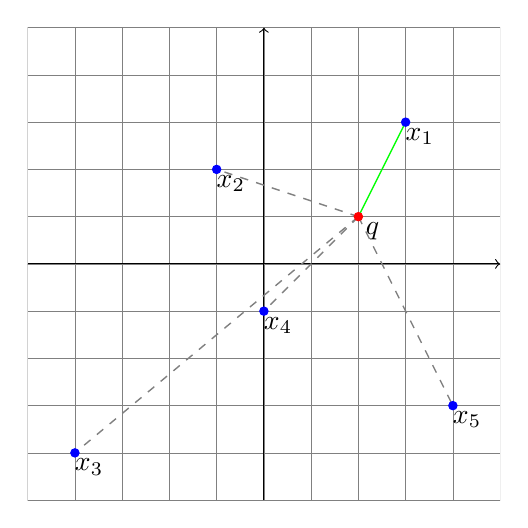
\begin{tikzpicture}[%
      scale=0.6,
      ]
      \clip (-5.0,-5.0) rectangle (5.0,5.0);
      \draw [help lines] (0,0) grid (6,5);
      \draw [help lines] (-6,0) grid (0,5);
      \draw [help lines] (0,-6) grid (6,0);
      \draw [help lines] (-6,-6) grid (0,0);
      \draw [color=black,->] (-5.0,0) -- (5.0,0);
      \draw [color=black,->] (0,-5.0) -- (0,5.0);
      
      \draw[color=green, line width=0.5pt, solid] (2,1) -- (3,3);
      \draw[color=gray, line width=0.5pt, dashed] (2,1) -- (-1,2);
      \draw[color=gray, line width=0.5pt, dashed] (2,1) -- (-4,-4);
      \draw[color=gray, line width=0.5pt, dashed] (2,1) -- (0,-1);
      \draw[color=gray, line width=0.5pt, dashed] (2,1) -- (4,-3);
      
      \filldraw [color={rgb:red,0;green,0;blue,255}] (3,3) circle (2.5pt );
      \filldraw [color={rgb:red,0;green,0;blue,255}] (-1,2) circle (2.5pt );
      \filldraw [color={rgb:red,0;green,0;blue,255}] (-4,-4) circle (2.5pt );
      \filldraw [color={rgb:red,0;green,0;blue,255}] (0,-1) circle (2.5pt );
      \filldraw [color={rgb:red,0;green,0;blue,255}] (4,-3) circle (2.5pt );
      
      \filldraw [color={rgb:red,255;green,0;blue,0}] (2,1) circle (2.5pt );
      
      \node at (3.3,2.7) {$x_1$};
      \node at (-0.7,1.7) {$x_2$};
      \node at (-3.7,-4.3) {$x_3$};
      \node at (0.3,-1.3) {$x_4$};
      \node at (4.3,-3.3) {$x_5$};
      
      \node at (2.3,0.7) {$q$};
      \end{tikzpicture}
  \end{column}
 \end{columns}
\end{frame}

% Vor- und Nachteile
\begin{frame}{Vollsuche}{Vor- und Nachteile}
 \begin{block}{Vorteile}
  \begin{itemize}
   \item Einfache Implementierung
   \item Funktioniert auch in Nicht-Metrischen R\"aumen
  \end{itemize}
 \end{block}
 \begin{block}{Nachteile}
  \begin{itemize}
   \item Hohe Laufzeiten gerade bei großen Datenmengen und h\"oherdimensionalen R\"aumen
  \end{itemize}
 \end{block}
\end{frame}

\begin{frame}{Metrik}
  Sei $X$ ein Menge. Unter einer \textit{Metrik} auf $X$ versteht man eine Abbildung\\
  $d:X \times X \to \mathbb{R}$, $(x, y) \mapsto d(x, y)$\\
  mit folgenden Eigenschaften:
 \begin{enumerate}
  \item $d(x, y) = 0$ genau dann, wenn $x=y$.
  \item Symmetrie: F\"ur alle $x, y \in X$ gilt $d(x, y) = d(y, x)$.
  \item Dreiecksungleichung: F\"ur alle $x, y, z \in X$ gilt $d(x, z) \le d(x, y) + d(y,z)$
 \end{enumerate}
 \flushright{\tiny{[Forster, 2006]}}
\end{frame}

\begin{frame}{Dreiecksungleichung}
 \textbf{Lemma} F\"ur beliebige $q, s, p \in \mathbb{U}$, $r \in \mathbb{R}$ und $P \subset \mathbb{U}$ gilt:
 \begin{enumerate}
  \item $|d(p, q) - d(p, s)| \le d(q, s) \le d(p, q) + d(p, s)$
  \item $d(q, s) \ge d_P(q, s) := \max_{p \in P}|d(p, q) - d(p, s)|$
  \item $d(p, s) > d(p, q) + r \vee d(p, s) < d(p, q) -r \Rightarrow d(q, s) > r$
  \item $d(p, s) \ge 2 \cdot d(p, q) \Rightarrow d(q, s) \ge d(q, p)$
 \end{enumerate}
 \flushright{\tiny{[Clarkson, 2005]}}
\end{frame}

\subsection{Orchard’s Algorithm}
\begin{frame}{Orchard’s Algorithm}
 \begin{itemize}
  \item Erstelle Liste f\"ur alle Punkt $p \in S$ mit allen Punkten $x \in S$, aufsteigenden nach ihrer Distanz
  \item W\"ahle zufälligen Punkt $c \in S$ als initialen Kandidaten
  \item Berechne $d(c, q)$
  \item Gehe Liste von $c$ entlange
  \item Wenn aktueller Punkt näher an $q$ als $c$, nimm aktuellen Punkt für $c$
  \item Abbruch, wenn
    \begin{itemize}
      \item die Liste komplett abgelaufen ist, oder
      \item $d(c, s) > 2 \cdot d(c, q)$ f\"ur aktuelles Element aus der Liste
    \end{itemize}
 \end{itemize}
\end{frame}

%Beispiel2
\begin{frame}{Orchard’s Algorithm}{Beispiel}
 \begin{columns}[T]
  \begin{column}{.35\textwidth}
    $\mathbb{U} = \mathbb{R}^2$
    \begin{block}{Datenpunkte}
      $x_1 = (3, 3)$\\
      $x_2 = (-1, 2)$\\
      $x_3 = (-4, -4)$\\
      $x_4 = (0, -1)$\\
      $x_5 = (4, -3)$
    \end{block}
    \begin{block}{Anfragepunkt}
      $q = (2, 1)$
    \end{block}
  \end{column}
  \begin{column}{.60\textwidth}
     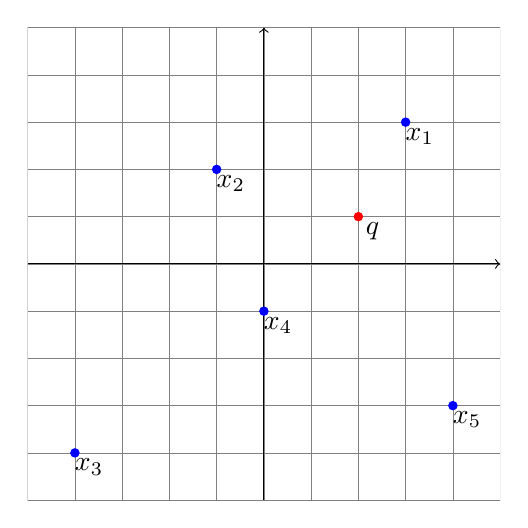
\begin{tikzpicture}[%
      scale=0.6,
      ]
      \clip (-5.0,-5.0) rectangle (5.0,5.0);
      \draw [help lines] (0,0) grid (6,5);
      \draw [help lines] (-6,0) grid (0,5);
      \draw [help lines] (0,-6) grid (6,0);
      \draw [help lines] (-6,-6) grid (0,0);
      \draw [color=black,->] (-5.0,0) -- (5.0,0);
      \draw [color=black,->] (0,-5.0) -- (0,5.0);
      
      \filldraw [color={rgb:red,0;green,0;blue,255}] (3,3) circle (2.5pt );
      \filldraw [color={rgb:red,0;green,0;blue,255}] (-1,2) circle (2.5pt );
      \filldraw [color={rgb:red,0;green,0;blue,255}] (-4,-4) circle (2.5pt );
      \filldraw [color={rgb:red,0;green,0;blue,255}] (0,-1) circle (2.5pt );
      \filldraw [color={rgb:red,0;green,0;blue,255}] (4,-3) circle (2.5pt );
      
      \filldraw [color={rgb:red,255;green,0;blue,0}] (2,1) circle (2.5pt );
      
      \node at (3.3,2.7) {$x_1$};
      \node at (-0.7,1.7) {$x_2$};
      \node at (-3.7,-4.3) {$x_3$};
      \node at (0.3,-1.3) {$x_4$};
      \node at (4.3,-3.3) {$x_5$};
      
      \node at (2.3,0.7) {$q$};
      \end{tikzpicture}
  \end{column}
 \end{columns}
\end{frame}

%Beispiel2 Listen
\begin{frame}{Orchard’s Algorithm}{Beispiel}
 \begin{columns}[T]
  \begin{column}{.35\textwidth}
    \begin{block}{Listen}
    $L(x_1) = \{x_2, x_4, x_5, x_3\}$\\
    $L(x_2) = \{x_4, x_1, x_3, x_5\}$\\
    $L(x_3) = \{x_4, x_2, x_5, x_1\}$\\
    $L(x_4) = \{x_2, x_5, x_1, x_3\}$\\
    $L(x_5) = \{x_4, x_1, x_2, x_3\}$\\
    \end{block}
  \end{column}
  \begin{column}{.6\textwidth}
     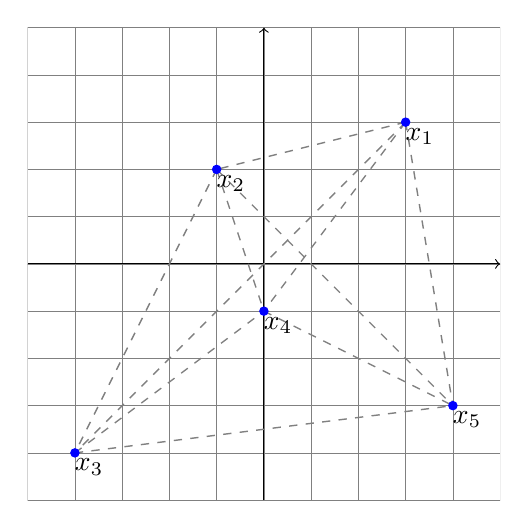
\begin{tikzpicture}[%
      scale=0.6,
      ]
      \clip (-5.0,-5.0) rectangle (5.0,5.0);
      \draw [help lines] (0,0) grid (6,5);
      \draw [help lines] (-6,0) grid (0,5);
      \draw [help lines] (0,-6) grid (6,0);
      \draw [help lines] (-6,-6) grid (0,0);
      \draw [color=black,->] (-5.0,0) -- (5.0,0);
      \draw [color=black,->] (0,-5.0) -- (0,5.0);
      
      \draw[color=gray, line width=0.5pt, dashed] (3,3) -- (-1,2);
      \draw[color=gray, line width=0.5pt, dashed] (3,3) -- (-4,-4);
      \draw[color=gray, line width=0.5pt, dashed] (3,3) -- (0,-1);
      \draw[color=gray, line width=0.5pt, dashed] (3,3) -- (4,-3);
      \draw[color=gray, line width=0.5pt, dashed] (-1,2) -- (-4,-4);
      \draw[color=gray, line width=0.5pt, dashed] (-1,2) -- (0,-1);
      \draw[color=gray, line width=0.5pt, dashed] (-1,2) -- (4,-3);
      \draw[color=gray, line width=0.5pt, dashed] (-4,-4) -- (0,-1);
      \draw[color=gray, line width=0.5pt, dashed] (-4,-4) -- (4,-3);
      \draw[color=gray, line width=0.5pt, dashed] (0,-1) -- (4,-3);
      
      \filldraw [color={rgb:red,0;green,0;blue,255}] (3,3) circle (2.5pt );
      \filldraw [color={rgb:red,0;green,0;blue,255}] (-1,2) circle (2.5pt );
      \filldraw [color={rgb:red,0;green,0;blue,255}] (-4,-4) circle (2.5pt );
      \filldraw [color={rgb:red,0;green,0;blue,255}] (0,-1) circle (2.5pt );
      \filldraw [color={rgb:red,0;green,0;blue,255}] (4,-3) circle (2.5pt );
      
      \node at (3.3,2.7) {$x_1$};
      \node at (-0.7,1.7) {$x_2$};
      \node at (-3.7,-4.3) {$x_3$};
      \node at (0.3,-1.3) {$x_4$};
      \node at (4.3,-3.3) {$x_5$};
      \end{tikzpicture}
  \end{column}
 \end{columns}
\end{frame}

%Beispiel2 Wähle c=x_3 und s=x_4
\begin{frame}{Orchard’s Algorithm}{Beispiel}
 \begin{columns}[T]
  \begin{column}{.35\textwidth}
    \begin{itemize}
     \item Setze $c:=x_3$ und $s:= x_4$
    \end{itemize}
  \end{column}
  \begin{column}{.60\textwidth}
     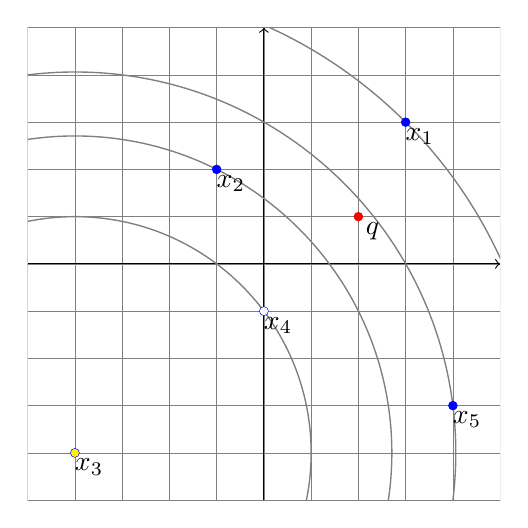
\begin{tikzpicture}[%
      scale=0.6,
      ]
      \clip (-5.0,-5.0) rectangle (5.0,5.0);
      \draw [help lines] (0,0) grid (6,5);
      \draw [help lines] (-6,0) grid (0,5);
      \draw [help lines] (0,-6) grid (6,0);
      \draw [help lines] (-6,-6) grid (0,0);
      \draw [color=black,->] (-5.0,0) -- (5.0,0);
      \draw [color=black,->] (0,-5.0) -- (0,5.0);
      
      \draw [color=gray, line width=0.5pt, solid] (-4,-4) circle (5);
      \draw [color=gray, line width=0.5pt, solid] (-4,-4) circle (6.708);
      \draw [color=gray, line width=0.5pt, solid] (-4,-4) circle (8.062);
      \draw [color=gray, line width=0.5pt, solid] (-4,-4) circle (9.899);
      \draw [color=yellow, line width=0.5pt, solid] (-4,-4) circle (15.62);
      
      \filldraw [color=blue] (3,3) circle (2.5pt );
      \filldraw [color=blue] (-1,2) circle (2.5pt );
      \filldraw [color=blue] (-4,-4) circle (2.5pt );
      \filldraw [color=yellow] (-4,-4) circle (2.1pt );
      \filldraw [color=blue] (0,-1) circle (2.5pt );
      \filldraw [color=white] (0,-1) circle (2.1pt );
      \filldraw [color=blue] (4,-3) circle (2.5pt );
      
      \filldraw [color=red] (2,1) circle (2.5pt );
      
      \node at (3.3,2.7) {$x_1$};
      \node at (-0.7,1.7) {$x_2$};
      \node at (-3.7,-4.3) {$x_3$};
      \node at (0.3,-1.3) {$x_4$};
      \node at (4.3,-3.3) {$x_5$};
      
      \node at (2.3,0.7) {$q$};
      \end{tikzpicture}
  \end{column}
 \end{columns}
\end{frame}

%Beispiel2 Wähle c=x_3 und s=x_4
\begin{frame}{Orchard’s Algorithm}{Beispiel}
 \begin{columns}[T]
  \begin{column}{.35\textwidth}
    \begin{itemize}
     \item Setze $c:=x_3$ und $s:= x_4$
     \item Da $7.810 \approx d(c, q) > d(s, q) \approx 2.828$, wird $x_4$ neues $c$
    \end{itemize}
  \end{column}
  \begin{column}{.60\textwidth}
     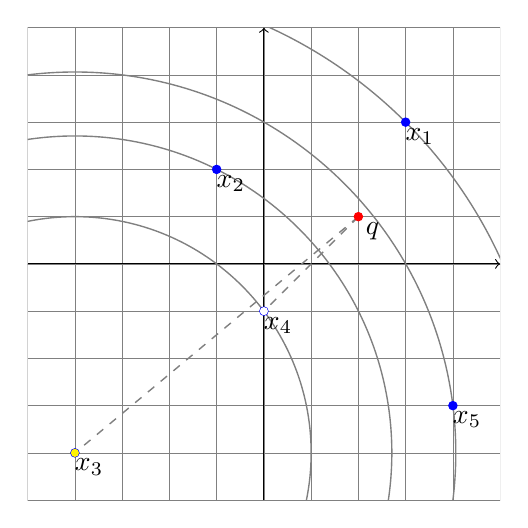
\begin{tikzpicture}[%
      scale=0.6,
      ]
      \clip (-5.0,-5.0) rectangle (5.0,5.0);
      \draw [help lines] (0,0) grid (6,5);
      \draw [help lines] (-6,0) grid (0,5);
      \draw [help lines] (0,-6) grid (6,0);
      \draw [help lines] (-6,-6) grid (0,0);
      \draw [color=black,->] (-5.0,0) -- (5.0,0);
      \draw [color=black,->] (0,-5.0) -- (0,5.0);
      
      \draw [color=gray, line width=0.5pt, solid] (-4,-4) circle (5);
      \draw [color=gray, line width=0.5pt, solid] (-4,-4) circle (6.708);
      \draw [color=gray, line width=0.5pt, solid] (-4,-4) circle (8.062);
      \draw [color=gray, line width=0.5pt, solid] (-4,-4) circle (9.899);
      \draw [color=yellow, line width=0.5pt, solid] (-4,-4) circle (15.62);
      \draw [color=yellow, line width=0.5pt, solid] (-4,-4) circle (15.62);
      
      \draw[color=gray, line width=0.5pt, dashed] (2,1) -- (-4,-4);
      \draw[color=gray, line width=0.5pt, dashed] (2,1) -- (0,-1);
      
      \filldraw [color=blue] (3,3) circle (2.5pt );
      \filldraw [color=blue] (-1,2) circle (2.5pt );
      \filldraw [color=blue] (-4,-4) circle (2.5pt );
      \filldraw [color=yellow] (-4,-4) circle (2.1pt );
      \filldraw [color=blue] (0,-1) circle (2.5pt );
      \filldraw [color=white] (0,-1) circle (2.1pt );
      \filldraw [color=blue] (4,-3) circle (2.5pt );
      
      \filldraw [color=red] (2,1) circle (2.5pt );
      
      \node at (3.3,2.7) {$x_1$};
      \node at (-0.7,1.7) {$x_2$};
      \node at (-3.7,-4.3) {$x_3$};
      \node at (0.3,-1.3) {$x_4$};
      \node at (4.3,-3.3) {$x_5$};
      
      \node at (2.3,0.7) {$q$};
      \end{tikzpicture}
  \end{column}
 \end{columns}
\end{frame}

%Beispiel2 Wähle c=x_4 und s=x_2
\begin{frame}{Orchard’s Algorithm}{Beispiel}
 \begin{columns}[T]
  \begin{column}{.35\textwidth}
    \begin{itemize}
     \item Setze $c:=x_4$ und $s:= x_2$
    \end{itemize}
  \end{column}
  \begin{column}{.60\textwidth}
     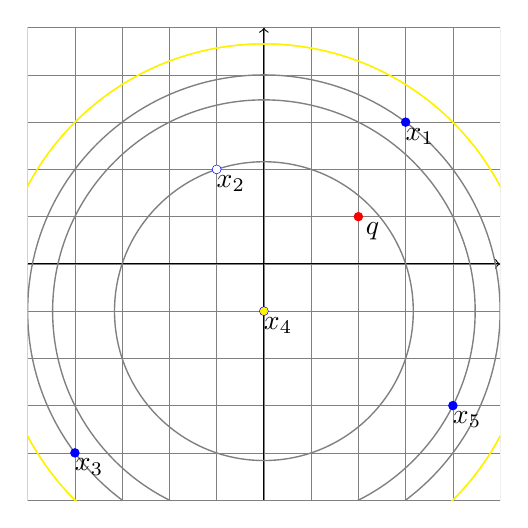
\begin{tikzpicture}[%
      scale=0.6,
      ]
      \clip (-5.0,-5.0) rectangle (5.0,5.0);
      \draw [help lines] (0,0) grid (6,5);
      \draw [help lines] (-6,0) grid (0,5);
      \draw [help lines] (0,-6) grid (6,0);
      \draw [help lines] (-6,-6) grid (0,0);
      \draw [color=black,->] (-5.0,0) -- (5.0,0);
      \draw [color=black,->] (0,-5.0) -- (0,5.0);
      
      \draw [color=gray, line width=0.5pt, solid] (0,-1) circle (3.162);
      \draw [color=gray, line width=0.5pt, solid] (0,-1) circle (4.472);
      \draw [color=gray, line width=0.5pt, solid] (0,-1) circle (5);
      \draw [color=yellow, line width=0.5pt, solid] (0,-1) circle (5.656);
      \draw [color=yellow, line width=0.5pt, solid] (0,-1) circle (5.656);
      
      \filldraw [color=blue] (3,3) circle (2.5pt );
      \filldraw [color=blue] (-1,2) circle (2.5pt );
      \filldraw [color=white] (-1,2) circle (2.1pt );
      \filldraw [color=blue] (-4,-4) circle (2.5pt );
      \filldraw [color=blue] (0,-1) circle (2.5pt );
      \filldraw [color=yellow] (0,-1) circle (2.1pt );
      \filldraw [color=blue] (4,-3) circle (2.5pt );
      
      \filldraw [color=red] (2,1) circle (2.5pt );
      
      \node at (3.3,2.7) {$x_1$};
      \node at (-0.7,1.7) {$x_2$};
      \node at (-3.7,-4.3) {$x_3$};
      \node at (0.3,-1.3) {$x_4$};
      \node at (4.3,-3.3) {$x_5$};
      
      \node at (2.3,0.7) {$q$};
      \end{tikzpicture}
  \end{column}
 \end{columns}
\end{frame}

%Beispiel2 Wähle c=x_4 und s=x_2
\begin{frame}{Orchard’s Algorithm}{Beispiel}
 \begin{columns}[T]
  \begin{column}{.35\textwidth}
    \begin{itemize}
     \item Setze $c:=x_4$ und $s:= x_2$
     \item Da $2.828 \approx d(c, q) < d(s, q) \approx 3.162$, kein neues $c$
    \end{itemize}
  \end{column}
  \begin{column}{.60\textwidth}
     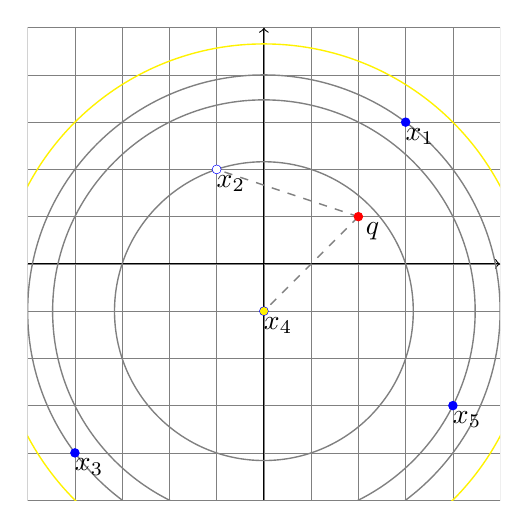
\begin{tikzpicture}[%
      scale=0.6,
      ]
      \clip (-5.0,-5.0) rectangle (5.0,5.0);
      \draw [help lines] (0,0) grid (6,5);
      \draw [help lines] (-6,0) grid (0,5);
      \draw [help lines] (0,-6) grid (6,0);
      \draw [help lines] (-6,-6) grid (0,0);
      \draw [color=black,->] (-5.0,0) -- (5.0,0);
      \draw [color=black,->] (0,-5.0) -- (0,5.0);
      
      \draw [color=gray, line width=0.5pt, solid] (0,-1) circle (3.162);
      \draw [color=gray, line width=0.5pt, solid] (0,-1) circle (4.472);
      \draw [color=gray, line width=0.5pt, solid] (0,-1) circle (5);
      \draw [color=yellow, line width=0.5pt, solid] (0,-1) circle (5.656);
      
      \draw[color=gray, line width=0.5pt, dashed] (2,1) -- (-1,2);
      \draw[color=gray, line width=0.5pt, dashed] (2,1) -- (0,-1);
      
      \filldraw [color=blue] (3,3) circle (2.5pt );
      \filldraw [color=blue] (-1,2) circle (2.5pt );
      \filldraw [color=white] (-1,2) circle (2.1pt );
      \filldraw [color=blue] (-4,-4) circle (2.5pt );
      \filldraw [color=blue] (0,-1) circle (2.5pt );
      \filldraw [color=yellow] (0,-1) circle (2.1pt );
      \filldraw [color=blue] (4,-3) circle (2.5pt );
      
      \filldraw [color=red] (2,1) circle (2.5pt );
      
      \node at (3.3,2.7) {$x_1$};
      \node at (-0.7,1.7) {$x_2$};
      \node at (-3.7,-4.3) {$x_3$};
      \node at (0.3,-1.3) {$x_4$};
      \node at (4.3,-3.3) {$x_5$};
      
      \node at (2.3,0.7) {$q$};
      \end{tikzpicture}
  \end{column}
 \end{columns}
\end{frame}

%Beispiel2 Wähle c=x_4 und s=x_2
\begin{frame}{Orchard’s Algorithm}{Beispiel}
 \begin{columns}[T]
  \begin{column}{.35\textwidth}
    \begin{itemize}
     \item Setze $c:=x_4$ und $s:= x_2$
     \item Da $2.828 \approx d(c, q) < d(s, q) \approx 3.162$, kein neues $c$
     \item Da $3.162 \approx d(c, s) < 2 \cdot d(c, q) \approx 5.656$, $x_4$ kein Abbruch
    \end{itemize}
  \end{column}
  \begin{column}{.60\textwidth}
     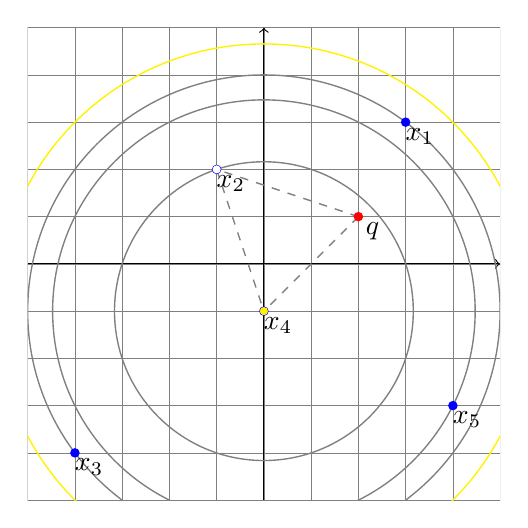
\begin{tikzpicture}[%
      scale=0.6,
      ]
      \clip (-5.0,-5.0) rectangle (5.0,5.0);
      \draw [help lines] (0,0) grid (6,5);
      \draw [help lines] (-6,0) grid (0,5);
      \draw [help lines] (0,-6) grid (6,0);
      \draw [help lines] (-6,-6) grid (0,0);
      \draw [color=black,->] (-5.0,0) -- (5.0,0);
      \draw [color=black,->] (0,-5.0) -- (0,5.0);
      
      \draw [color=gray, line width=0.5pt, solid] (0,-1) circle (3.162);
      \draw [color=gray, line width=0.5pt, solid] (0,-1) circle (4.472);
      \draw [color=gray, line width=0.5pt, solid] (0,-1) circle (5);
      \draw [color=yellow, line width=0.5pt, solid] (0,-1) circle (5.656);
      
      \draw[color=gray, line width=0.5pt, dashed] (2,1) -- (-1,2);
      \draw[color=gray, line width=0.5pt, dashed] (2,1) -- (0,-1);
      \draw[color=gray, line width=0.5pt, dashed] (-1,2) -- (0,-1);
      
      \filldraw [color=blue] (3,3) circle (2.5pt );
      \filldraw [color=blue] (-1,2) circle (2.5pt );
      \filldraw [color=white] (-1,2) circle (2.1pt );
      \filldraw [color=blue] (-4,-4) circle (2.5pt );
      \filldraw [color=blue] (0,-1) circle (2.5pt );
      \filldraw [color=yellow] (0,-1) circle (2.1pt );
      \filldraw [color=blue] (4,-3) circle (2.5pt );
      
      \filldraw [color=red] (2,1) circle (2.5pt );
      
      \node at (3.3,2.7) {$x_1$};
      \node at (-0.7,1.7) {$x_2$};
      \node at (-3.7,-4.3) {$x_3$};
      \node at (0.3,-1.3) {$x_4$};
      \node at (4.3,-3.3) {$x_5$};
      
      \node at (2.3,0.7) {$q$};
      \end{tikzpicture}
  \end{column}
 \end{columns}
\end{frame}

%Beispiel2 Wähle c=x_4 und s=x_5
\begin{frame}{Orchard’s Algorithm}{Beispiel}
 \begin{columns}[T]
  \begin{column}{.35\textwidth}
    \begin{itemize}
     \item Setze $s:= x_5$
    \end{itemize}
  \end{column}
  \begin{column}{.60\textwidth}
     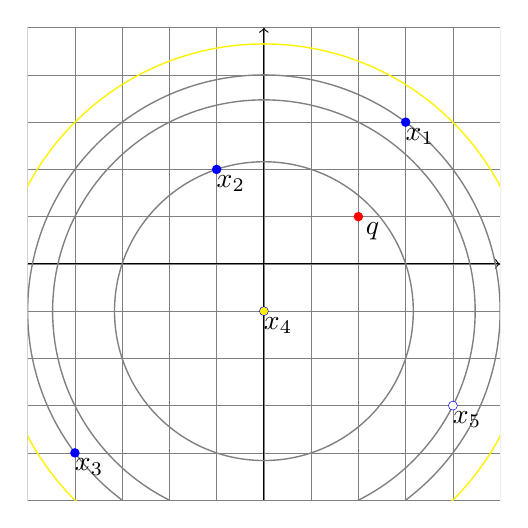
\begin{tikzpicture}[%
      scale=0.6,
      ]
      \clip (-5.0,-5.0) rectangle (5.0,5.0);
      \draw [help lines] (0,0) grid (6,5);
      \draw [help lines] (-6,0) grid (0,5);
      \draw [help lines] (0,-6) grid (6,0);
      \draw [help lines] (-6,-6) grid (0,0);
      \draw [color=black,->] (-5.0,0) -- (5.0,0);
      \draw [color=black,->] (0,-5.0) -- (0,5.0);
      
      \draw [color=gray, line width=0.5pt, solid] (0,-1) circle (3.162);
      \draw [color=gray, line width=0.5pt, solid] (0,-1) circle (4.472);
      \draw [color=gray, line width=0.5pt, solid] (0,-1) circle (5);
      \draw [color=yellow, line width=0.5pt, solid] (0,-1) circle (5.656);
      
      \filldraw [color=blue] (3,3) circle (2.5pt );
      \filldraw [color=blue] (-1,2) circle (2.5pt );
      \filldraw [color=blue] (-4,-4) circle (2.5pt );
      \filldraw [color=blue] (0,-1) circle (2.5pt );
      \filldraw [color=yellow] (0,-1) circle (2.1pt );
      \filldraw [color=blue] (4,-3) circle (2.5pt );
      \filldraw [color=white] (4,-3) circle (2.1pt );
      
      \filldraw [color=red] (2,1) circle (2.5pt );
      
      \node at (3.3,2.7) {$x_1$};
      \node at (-0.7,1.7) {$x_2$};
      \node at (-3.7,-4.3) {$x_3$};
      \node at (0.3,-1.3) {$x_4$};
      \node at (4.3,-3.3) {$x_5$};
      
      \node at (2.3,0.7) {$q$};
      \end{tikzpicture}
  \end{column}
 \end{columns}
\end{frame}

%Beispiel2 Wähle c=x_4 und s=x_5
\begin{frame}{Orchard’s Algorithm}{Beispiel}
 \begin{columns}[T]
  \begin{column}{.35\textwidth}
    \begin{itemize}
     \item Setze $s:= x_5$
     \item Da $2.828 \approx d(c, q) < d(s, q) \approx 4.472$, kein neues $c$
    \end{itemize}
  \end{column}
  \begin{column}{.60\textwidth}
     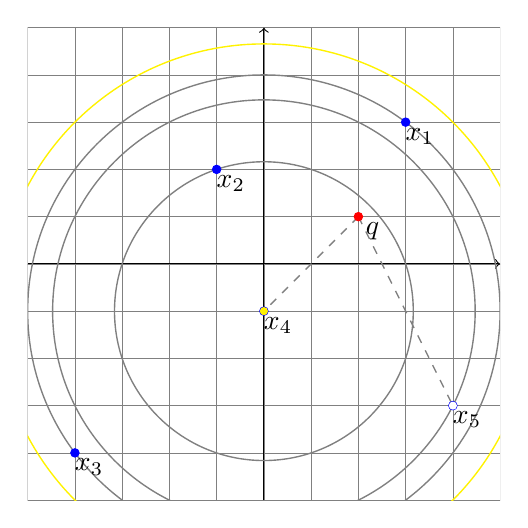
\begin{tikzpicture}[%
      scale=0.6,
      ]
      \clip (-5.0,-5.0) rectangle (5.0,5.0);
      \draw [help lines] (0,0) grid (6,5);
      \draw [help lines] (-6,0) grid (0,5);
      \draw [help lines] (0,-6) grid (6,0);
      \draw [help lines] (-6,-6) grid (0,0);
      \draw [color=black,->] (-5.0,0) -- (5.0,0);
      \draw [color=black,->] (0,-5.0) -- (0,5.0);
      
      \draw [color=gray, line width=0.5pt, solid] (0,-1) circle (3.162);
      \draw [color=gray, line width=0.5pt, solid] (0,-1) circle (4.472);
      \draw [color=gray, line width=0.5pt, solid] (0,-1) circle (5);
      \draw [color=yellow, line width=0.5pt, solid] (0,-1) circle (5.656);
      
      \draw[color=gray, line width=0.5pt, dashed] (2,1) -- (4,-3);
      \draw[color=gray, line width=0.5pt, dashed] (2,1) -- (0,-1);
      
      \filldraw [color=blue] (3,3) circle (2.5pt );
      \filldraw [color=blue] (-1,2) circle (2.5pt );
      \filldraw [color=blue] (-4,-4) circle (2.5pt );
      \filldraw [color=blue] (0,-1) circle (2.5pt );
      \filldraw [color=yellow] (0,-1) circle (2.1pt );
      \filldraw [color=blue] (4,-3) circle (2.5pt );
      \filldraw [color=white] (4,-3) circle (2.1pt );
      
      \filldraw [color=red] (2,1) circle (2.5pt );
      
      \node at (3.3,2.7) {$x_1$};
      \node at (-0.7,1.7) {$x_2$};
      \node at (-3.7,-4.3) {$x_3$};
      \node at (0.3,-1.3) {$x_4$};
      \node at (4.3,-3.3) {$x_5$};
      
      \node at (2.3,0.7) {$q$};
      \end{tikzpicture}
  \end{column}
 \end{columns}
\end{frame}

%Beispiel2 Wähle c=x_4 und s=x_5
\begin{frame}{Orchard’s Algorithm}{Beispiel}
 \begin{columns}[T]
  \begin{column}{.35\textwidth}
    \begin{itemize}
     \item Setze $s:= x_5$
     \item Da $2.828 \approx d(c, q) < d(s, q) \approx 4.472$, kein neues $c$
     \item Da $4.472 \approx d(c, s) < 2 \cdot d(c, q) \approx 5.656$, $x_4$ kein Abbruch
    \end{itemize}
  \end{column}
  \begin{column}{.60\textwidth}
     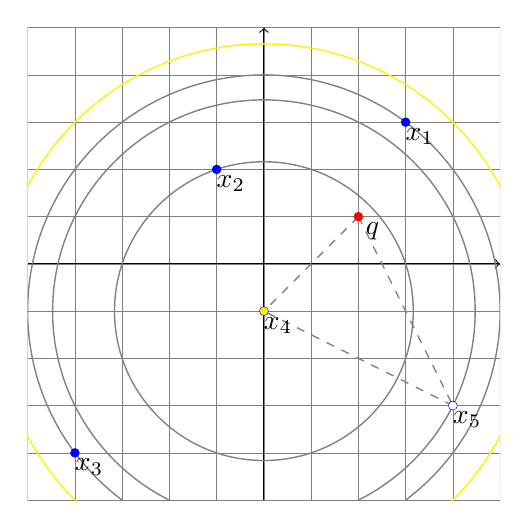
\begin{tikzpicture}[%
      scale=0.6,
      ]
      \clip (-5.0,-5.0) rectangle (5.0,5.0);
      \draw [help lines] (0,0) grid (6,5);
      \draw [help lines] (-6,0) grid (0,5);
      \draw [help lines] (0,-6) grid (6,0);
      \draw [help lines] (-6,-6) grid (0,0);
      \draw [color=black,->] (-5.0,0) -- (5.0,0);
      \draw [color=black,->] (0,-5.0) -- (0,5.0);
      
      \draw [color=gray, line width=0.5pt, solid] (0,-1) circle (3.162);
      \draw [color=gray, line width=0.5pt, solid] (0,-1) circle (4.472);
      \draw [color=gray, line width=0.5pt, solid] (0,-1) circle (5);
      \draw [color=yellow, line width=0.5pt, solid] (0,-1) circle (5.656);
      
      \draw[color=gray, line width=0.5pt, dashed] (2,1) -- (4,-3);
      \draw[color=gray, line width=0.5pt, dashed] (2,1) -- (0,-1);
      \draw[color=gray, line width=0.5pt, dashed] (4,-3) -- (0,-1);
      
      \filldraw [color=blue] (3,3) circle (2.5pt );
      \filldraw [color=blue] (-1,2) circle (2.5pt );
      \filldraw [color=blue] (-4,-4) circle (2.5pt );
      \filldraw [color=blue] (0,-1) circle (2.5pt );
      \filldraw [color=yellow] (0,-1) circle (2.1pt );
      \filldraw [color=blue] (4,-3) circle (2.5pt );
      \filldraw [color=white] (4,-3) circle (2.1pt );
      
      \filldraw [color=red] (2,1) circle (2.5pt );
      
      \node at (3.3,2.7) {$x_1$};
      \node at (-0.7,1.7) {$x_2$};
      \node at (-3.7,-4.3) {$x_3$};
      \node at (0.3,-1.3) {$x_4$};
      \node at (4.3,-3.3) {$x_5$};
      
      \node at (2.3,0.7) {$q$};
      \end{tikzpicture}
  \end{column}
 \end{columns}
\end{frame}

%Beispiel2 Wähle c=x_4 und s=x_1
\begin{frame}{Orchard’s Algorithm}{Beispiel}
 \begin{columns}[T]
  \begin{column}{.35\textwidth}
    \begin{itemize}
     \item Setze $s:= x_1$
    \end{itemize}
  \end{column}
  \begin{column}{.60\textwidth}
     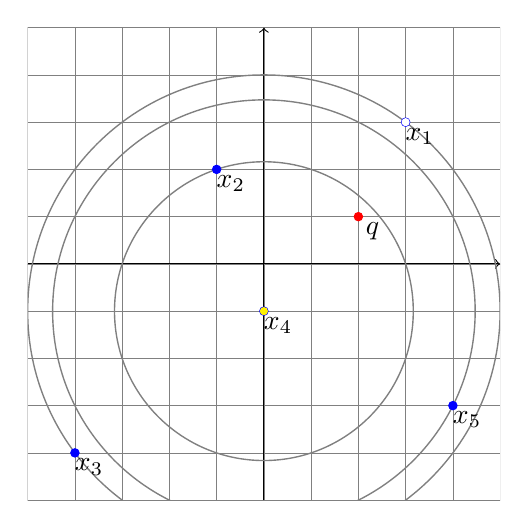
\begin{tikzpicture}[%
      scale=0.6,
      ]
      \clip (-5.0,-5.0) rectangle (5.0,5.0);
      \draw [help lines] (0,0) grid (6,5);
      \draw [help lines] (-6,0) grid (0,5);
      \draw [help lines] (0,-6) grid (6,0);
      \draw [help lines] (-6,-6) grid (0,0);
      \draw [color=black,->] (-5.0,0) -- (5.0,0);
      \draw [color=black,->] (0,-5.0) -- (0,5.0);
      
      \draw [color=gray, line width=0.5pt, solid] (0,-1) circle (3.162);
      \draw [color=gray, line width=0.5pt, solid] (0,-1) circle (4.472);
      \draw [color=gray, line width=0.5pt, solid] (0,-1) circle (5);
      
      \filldraw [color=blue] (3,3) circle (2.5pt );
      \filldraw [color=white] (3,3) circle (2.1pt );
      \filldraw [color=blue] (-1,2) circle (2.5pt );
      \filldraw [color=blue] (-4,-4) circle (2.5pt );
      \filldraw [color=blue] (0,-1) circle (2.5pt );
      \filldraw [color=yellow] (0,-1) circle (2.1pt );
      \filldraw [color=blue] (4,-3) circle (2.5pt );
      
      \filldraw [color=red] (2,1) circle (2.5pt );
      
      \node at (3.3,2.7) {$x_1$};
      \node at (-0.7,1.7) {$x_2$};
      \node at (-3.7,-4.3) {$x_3$};
      \node at (0.3,-1.3) {$x_4$};
      \node at (4.3,-3.3) {$x_5$};
      
      \node at (2.3,0.7) {$q$};
      \end{tikzpicture}
  \end{column}
 \end{columns}
\end{frame}

%Beispiel2 Wähle c=x_4 und s=x_1
\begin{frame}{Orchard’s Algorithm}{Beispiel}
 \begin{columns}[T]
  \begin{column}{.35\textwidth}
    \begin{itemize}
     \item Setze $s:= x_1$
     \item Da $2.828 \approx d(c, q) > d(s, q) \approx 2.236$, wird $x_1$ neues $c$
    \end{itemize}
  \end{column}
  \begin{column}{.60\textwidth}
     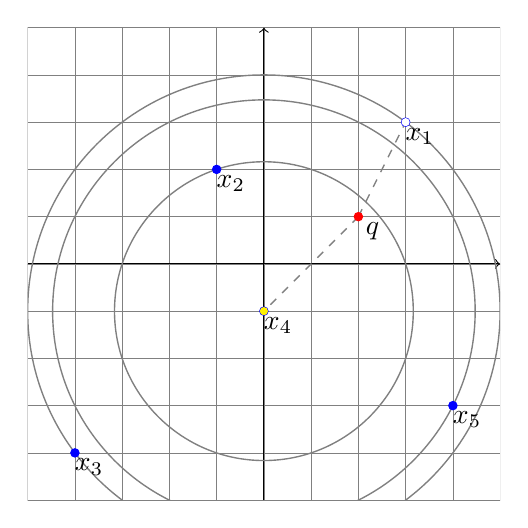
\begin{tikzpicture}[%
      scale=0.6,
      ]
      \clip (-5.0,-5.0) rectangle (5.0,5.0);
      \draw [help lines] (0,0) grid (6,5);
      \draw [help lines] (-6,0) grid (0,5);
      \draw [help lines] (0,-6) grid (6,0);
      \draw [help lines] (-6,-6) grid (0,0);
      \draw [color=black,->] (-5.0,0) -- (5.0,0);
      \draw [color=black,->] (0,-5.0) -- (0,5.0);
      
      \draw [color=gray, line width=0.5pt, solid] (0,-1) circle (3.162);
      \draw [color=gray, line width=0.5pt, solid] (0,-1) circle (4.472);
      \draw [color=gray, line width=0.5pt, solid] (0,-1) circle (5);
      
      \draw[color=gray, line width=0.5pt, dashed] (2,1) -- (3,3);
      \draw[color=gray, line width=0.5pt, dashed] (2,1) -- (0,-1);
      
      \filldraw [color=blue] (3,3) circle (2.5pt );
      \filldraw [color=white] (3,3) circle (2.1pt );
      \filldraw [color=blue] (-1,2) circle (2.5pt );
      \filldraw [color=blue] (-4,-4) circle (2.5pt );
      \filldraw [color=blue] (0,-1) circle (2.5pt );
      \filldraw [color=yellow] (0,-1) circle (2.1pt );
      \filldraw [color=blue] (4,-3) circle (2.5pt );
      
      \filldraw [color=red] (2,1) circle (2.5pt );
      
      \node at (3.3,2.7) {$x_1$};
      \node at (-0.7,1.7) {$x_2$};
      \node at (-3.7,-4.3) {$x_3$};
      \node at (0.3,-1.3) {$x_4$};
      \node at (4.3,-3.3) {$x_5$};
      
      \node at (2.3,0.7) {$q$};
      \end{tikzpicture}
  \end{column}
 \end{columns}
\end{frame}

%Beispiel2 Wähle c=x_1 und s=x_2
\begin{frame}{Orchard’s Algorithm}{Beispiel}
 \begin{columns}[T]
  \begin{column}{.35\textwidth}
    \begin{itemize}
     \item Setze $c:= x_1$ und $s:=x_2$
    \end{itemize}
  \end{column}
  \begin{column}{.60\textwidth}
     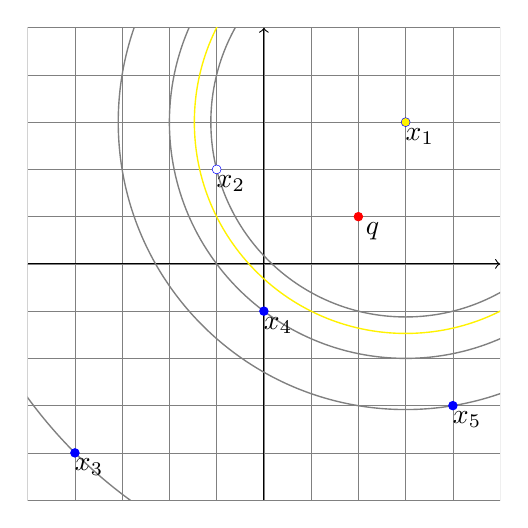
\begin{tikzpicture}[%
      scale=0.6,
      ]
      \clip (-5.0,-5.0) rectangle (5.0,5.0);
      \draw [help lines] (0,0) grid (6,5);
      \draw [help lines] (-6,0) grid (0,5);
      \draw [help lines] (0,-6) grid (6,0);
      \draw [help lines] (-6,-6) grid (0,0);
      \draw [color=black,->] (-5.0,0) -- (5.0,0);
      \draw [color=black,->] (0,-5.0) -- (0,5.0);
      
      \draw [color=gray, line width=0.5pt, solid] (3,3) circle (4.123);
      \draw [color=gray, line width=0.5pt, solid] (3,3) circle (5);
      \draw [color=gray, line width=0.5pt, solid] (3,3) circle (6.083);
      \draw [color=gray, line width=0.5pt, solid] (3,3) circle (9.899);
      \draw [color=yellow, line width=0.5pt, solid] (3,3) circle (4.472);
      
      \filldraw [color=blue] (3,3) circle (2.5pt );
      \filldraw [color=yellow] (3,3) circle (2.1pt );
      \filldraw [color=blue] (-1,2) circle (2.5pt );
      \filldraw [color=white] (-1,2) circle (2.1pt );
      \filldraw [color=blue] (-4,-4) circle (2.5pt );
      \filldraw [color=blue] (0,-1) circle (2.5pt );
      \filldraw [color=blue] (4,-3) circle (2.5pt );
      
      \filldraw [color=red] (2,1) circle (2.5pt );
      
      \node at (3.3,2.7) {$x_1$};
      \node at (-0.7,1.7) {$x_2$};
      \node at (-3.7,-4.3) {$x_3$};
      \node at (0.3,-1.3) {$x_4$};
      \node at (4.3,-3.3) {$x_5$};
      
      \node at (2.3,0.7) {$q$};
      \end{tikzpicture}
  \end{column}
 \end{columns}
\end{frame}

%Beispiel2 Wähle c=x_1 und s=x_2
\begin{frame}{Orchard’s Algorithm}{Beispiel}
 \begin{columns}[T]
  \begin{column}{.35\textwidth}
    \begin{itemize}
     \item Setze $c:= x_1$ und $s:=x_2$
     \item Da $2.236 \approx d(c, q) < d(s, q) \approx 3.162$, kein neues $c$
    \end{itemize}
  \end{column}
  \begin{column}{.60\textwidth}
     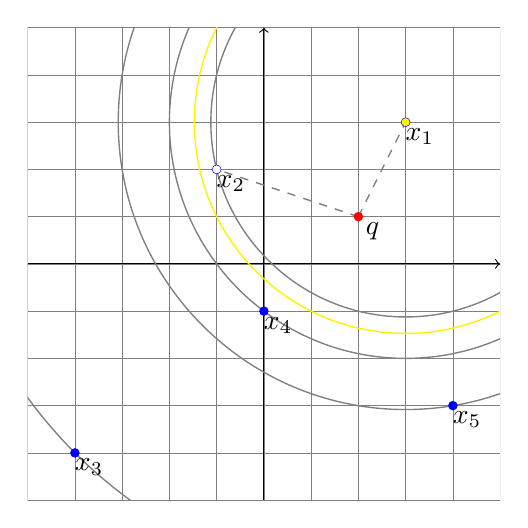
\begin{tikzpicture}[%
      scale=0.6,
      ]
      \clip (-5.0,-5.0) rectangle (5.0,5.0);
      \draw [help lines] (0,0) grid (6,5);
      \draw [help lines] (-6,0) grid (0,5);
      \draw [help lines] (0,-6) grid (6,0);
      \draw [help lines] (-6,-6) grid (0,0);
      \draw [color=black,->] (-5.0,0) -- (5.0,0);
      \draw [color=black,->] (0,-5.0) -- (0,5.0);
      
      \draw [color=gray, line width=0.5pt, solid] (3,3) circle (4.123);
      \draw [color=gray, line width=0.5pt, solid] (3,3) circle (5);
      \draw [color=gray, line width=0.5pt, solid] (3,3) circle (6.083);
      \draw [color=gray, line width=0.5pt, solid] (3,3) circle (9.899);
      \draw [color=yellow, line width=0.5pt, solid] (3,3) circle (4.472);
      
      \draw[color=gray, line width=0.5pt, dashed] (2,1) -- (3,3);
      \draw[color=gray, line width=0.5pt, dashed] (2,1) -- (-1,2);
      
      \filldraw [color=blue] (3,3) circle (2.5pt );
      \filldraw [color=yellow] (3,3) circle (2.1pt );
      \filldraw [color=blue] (-1,2) circle (2.5pt );
      \filldraw [color=white] (-1,2) circle (2.1pt );
      \filldraw [color=blue] (-4,-4) circle (2.5pt );
      \filldraw [color=blue] (0,-1) circle (2.5pt );
      \filldraw [color=blue] (4,-3) circle (2.5pt );
      
      \filldraw [color=red] (2,1) circle (2.5pt );
      
      \node at (3.3,2.7) {$x_1$};
      \node at (-0.7,1.7) {$x_2$};
      \node at (-3.7,-4.3) {$x_3$};
      \node at (0.3,-1.3) {$x_4$};
      \node at (4.3,-3.3) {$x_5$};
      
      \node at (2.3,0.7) {$q$};
      \end{tikzpicture}
  \end{column}
 \end{columns}
\end{frame}

%Beispiel2 Wähle c=x_1 und s=x_2
\begin{frame}{Orchard’s Algorithm}{Beispiel}
 \begin{columns}[T]
  \begin{column}{.35\textwidth}
    \begin{itemize}
     \item Setze $c:= x_1$ und $s:=x_2$
     \item Da $2.236 \approx d(c, q) < d(s, q) \approx 3.162$, kein neues $c$
     \item Da $4.123 \approx d(c, s) < 2 \cdot d(c, q) \approx 4.472$, $x_4$ kein Abbruch
    \end{itemize}
  \end{column}
  \begin{column}{.60\textwidth}
     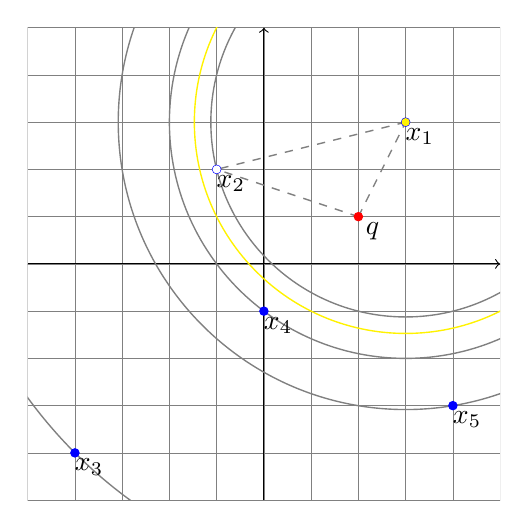
\begin{tikzpicture}[%
      scale=0.6,
      ]
      \clip (-5.0,-5.0) rectangle (5.0,5.0);
      \draw [help lines] (0,0) grid (6,5);
      \draw [help lines] (-6,0) grid (0,5);
      \draw [help lines] (0,-6) grid (6,0);
      \draw [help lines] (-6,-6) grid (0,0);
      \draw [color=black,->] (-5.0,0) -- (5.0,0);
      \draw [color=black,->] (0,-5.0) -- (0,5.0);
      
      \draw [color=gray, line width=0.5pt, solid] (3,3) circle (4.123);
      \draw [color=gray, line width=0.5pt, solid] (3,3) circle (5);
      \draw [color=gray, line width=0.5pt, solid] (3,3) circle (6.083);
      \draw [color=gray, line width=0.5pt, solid] (3,3) circle (9.899);
      \draw [color=yellow, line width=0.5pt, solid] (3,3) circle (4.472);
      
      \draw[color=gray, line width=0.5pt, dashed] (2,1) -- (3,3);
      \draw[color=gray, line width=0.5pt, dashed] (2,1) -- (-1,2);
      \draw[color=gray, line width=0.5pt, dashed] (3,3) -- (-1,2);
      
      \filldraw [color=blue] (3,3) circle (2.5pt );
      \filldraw [color=yellow] (3,3) circle (2.1pt );
      \filldraw [color=blue] (-1,2) circle (2.5pt );
      \filldraw [color=white] (-1,2) circle (2.1pt );
      \filldraw [color=blue] (-4,-4) circle (2.5pt );
      \filldraw [color=blue] (0,-1) circle (2.5pt );
      \filldraw [color=blue] (4,-3) circle (2.5pt );
      
      \filldraw [color=red] (2,1) circle (2.5pt );
      
      \node at (3.3,2.7) {$x_1$};
      \node at (-0.7,1.7) {$x_2$};
      \node at (-3.7,-4.3) {$x_3$};
      \node at (0.3,-1.3) {$x_4$};
      \node at (4.3,-3.3) {$x_5$};
      
      \node at (2.3,0.7) {$q$};
      \end{tikzpicture}
  \end{column}
 \end{columns}
\end{frame}

\section{Quellen}
\begin{frame}
 \frametitle{Quellen}
 \begin{itemize}
  \item Otto Forster, 2006, \textit{Analysis 2}, Friedr. Vieweg \& Sohn Verlag
  \item Kenneth L. Clarkson, 2005, \textit{Nearest-Neighbor Searching and Metric Space Dimensions}, http://kenclarkson.org/nn\_survey/p.pdf
  \end{itemize}
\end{frame}

\end{document}
